\documentclass{sigchi}

% Use this command to override the default ACM copyright statement (e.g. for preprints). 
% Consult the conference website for the camera-ready copyright statement.


% EXAMPLE BEGIN -- HOW TO OVERRIDE THE DEFAULT COPYRIGHT STRIP -- (July 22, 2013 - Paul Baumann)
 \toappear{Permission to make digital or hard copies of all or part of this work for personal or classroom use is granted without fee provided that copies are not made or distributed for profit or commercial advantage and that copies bear this notice and the full citation on the first page. Copyrights for components of this work owned by others than ACM must be honored. Abstracting with credit is permitted. To copy otherwise, or republish, to post on servers or to redistribute to lists, requires prior specific permission and/or a fee. Request permissions from permissions@acm.org. \\
 {\emph{CHI'14}}, April 26--May 1, 2014, Toronto, Canada. \\
 Copyright \copyright~2014 ACM ISBN/14/04...\$15.00. \\
 DOI string from ACM form confirmation}
% EXAMPLE END -- HOW TO OVERRIDE THE DEFAULT COPYRIGHT STRIP -- (July 22, 2013 - Paul Baumann)


% Arabic page numbers for submission. 
% Remove this line to eliminate page numbers for the camera ready copy
\pagenumbering{arabic}


% Load basic packages
\usepackage{balance}  % to better equalize the last page
\usepackage{graphics} % for EPS, load graphicx instead
\usepackage{times}    % comment if you want LaTeX's default font
\usepackage{url}      % llt: nicely formatted URLs

% llt: Define a global style for URLs, rather that the default one
\makeatletter
\def\url@leostyle{%
  \@ifundefined{selectfont}{\def\UrlFont{\sf}}{\def\UrlFont{\small\bf\ttfamily}}}
\makeatother
\urlstyle{leo}


% To make various LaTeX processors do the right thing with page size.
\def\pprw{8.5in}
\def\pprh{11in}
\special{papersize=\pprw,\pprh}
\setlength{\paperwidth}{\pprw}
\setlength{\paperheight}{\pprh}
\setlength{\pdfpagewidth}{\pprw}
\setlength{\pdfpageheight}{\pprh}

% Make sure hyperref comes last of your loaded packages, 
% to give it a fighting chance of not being over-written, 
% since its job is to redefine many LaTeX commands.
\usepackage[pdftex]{hyperref}
\hypersetup{
pdftitle={SIGCHI Conference Proceedings Format},
pdfauthor={LaTeX},
pdfkeywords={SIGCHI, proceedings, archival format},
bookmarksnumbered,
pdfstartview={FitH},
colorlinks,
citecolor=black,
filecolor=black,
linkcolor=black,
urlcolor=black,
breaklinks=true,
}

% create a shortcut to typeset table headings
\newcommand\tabhead[1]{\small\textbf{#1}}


% End of preamble. Here it comes the document.
\begin{document}

\title{MindMargin: Capturing Reader Engagement with an Article-Adjacent Commenting Platform}

\numberofauthors{3}
\author{
  \alignauthor Daniel Haehn\\
    \affaddr{Harvard University}\\
    \affaddr{Cambridge, MA, USA}\\
    \email{haehn@seas.harvard.edu}\\
    \affaddr{}
  \alignauthor Sharon Zhou\\
    \affaddr{Harvard University}\\
    \affaddr{Cambridge, MA, USA}\\
    \email{zhou12@college.harvard.edu}\\
    \affaddr{}    
  \alignauthor 3rd Author Name\\
    \affaddr{Affiliation}\\
    \affaddr{Address}\\
    \email{e-mail address}\\
    \affaddr{Optional phone number}
}

\maketitle

\begin{abstract}
Commenting systems are popular throughout many websites. Reading and writing comments can support passive consumption of media by increasing active user engagement in many ways. Information exchange, personal reflection, and lively discussion are only some possible outcomes. We explore how user engagement can be increased by proposing a new commenting system and interface, MindMargin. In contrast to traditional commenting systems where comments are featured below the article, MindMargin presents comments adjacent to its reference media. Users can post and navigate comments and replies on a horizontal infinite scroll. This exposes users to a diverse array of opinions as they read since comments in our system are anchored to relevant areas of the article. 

Furthermore, we propose a novel metric for classifying and more visibly displaying "popular" comments. Our metric includes the number of up- and down-votes as well as the post time. This guarantees that new comments are visible even if many popular comments already populate the article.

We define three hypotheses to measure increased user engagement that A) investigate if article-adjacent comments generate more comments, B) explore if permanent exposure to comments while reading impacts individual stance towards an issue or opinion in the article, and C) measure the influence of article-adjacent comments on a reader's impression of the comments. From a user study with 46 young adults, we accepted the second and third hypotheses. We explain the rejection of the first hypothesis as a result of various factors, including the novelty effect. We also discuss how the rejection of our first hypothesis coupled with acceptance of our second and third, in fact, further support our conclusions on increased reader engagement in MindMargin.

Based on our initial evaluation and results, we have concluded that the proposed MindMargin system is superior to traditional commenting systems in increasing user engagement while reading articles.
\end{abstract}

\keywords{
	Comments; commenting system; anchored; user engagement.
}

%\category{H.5.2.}{Information Interfaces and Presentation (e.g. HCI)}{User Interfaces}

\section{Introduction}

News pages, media sites, online shops, blogs and social networks support the ability to give content-related feedback in the form of comments. Commenting systems on these sites are traditionally featured under, and separate from, the main content. This structure parallels the relationship between content and comments, as interactions with comments are markedly secondary to the primary task of reading or browsing primary content. However, studies on Fluid Documents and annotation interfaces that challenge typographic conventions, such as discussion boards and footnotes, reveal limitations in the traditional vertical interface and suggest alternative horizontal layouts~\cite{FluidDocs,NewsInterfaces,NB,AnnotationsStudents,Brush,Guzdial,van}. 

The Fluid Documents project aims to make information added into a page easier to locate in its source document by adjusting the typography of page. One specific study found that a fluid margin interface, as opposed to a fluid interline or overlay interface, had minimal disturbance to the user, because it did not move or occlude the primary text with the secondary text~\cite{FluidDocs}. 

The concept of anchoring annotations to references in a text has been known to qualitatively improve conversation among readers because it makes understanding the context of a comment cognitively easier~\cite{Brush,Guzdial,van}. Another study compares the four leading annotation interfaces: footnotes, interlinear commentary, ``sticky-note`` annotations, and marginal comments, concluding that the marginal interface is superior in minimizing distraction and enhancing visibility. The marginal interfaces studied, however, interact with the primary text. They are tagged to boxes around the referenced content to indicate where they are anchored~\cite{AnnotationsStudents}. 

We have thus chosen to anchor comments in MindMargin with a faint dotted line to the edge of the article that corresponds to the y-coordinate of its reference, yet still avoids disturbing the primary text.

While online commenting provides an opportunity for readers to express their views and engage in lively discussion with others, the comments section of many websites has become a popular space for “flame wars.” The social act of “flaming,” or the posting of offensive content, regularly devolves into hostile fights among multiple users, diverting a legitimate discussion topic to an unrelated and often emotionally charged digression. This behavior is examined closely in many research fields, including user interface design, communications, and psychology~\cite{FlamingComp,FlamingPsych,FlamingSoftware,FlamingCommunications}. 

Evidence in educational research, however, has shown that anchored annotated notes foster a deeper understanding of the text and facilitate more thoughtful teacher-to-student and peer-to-peer discussions~\cite{AnnotationsStudents,NB}. Studies on balancing people’s skewed opinions also suggest exposing readers to a variety of relevant perspectives so that they consider views that exist beyond a single article and author’s scope~\cite{Politics,NewsCube,ConsiderIt}. 

Thus, while current commenting platforms often fail at drawing people into sensible and relevant conversation, we offer evidence to suggest a horizontal interface such as MindMargin can change people’s views and actions, and thus address this societal problem. From our evaluation and user study, it appears that people with prior exposure to the issue in the article become more moderate in their opinions, reporting less polar views than those using a traditional vertical interface.

\subsection{Hypotheses}
We propose two hypotheses for MindMargin's effect on its users in comparison to the traditional vertical interface:
\begin{enumerate}
\item Users of MindMargin will develop more thoughtful and nuanced opinions of an article, because MindMargin encourages readers to consider alternate views by exposing them to a greater diversity and number of comments.
\item Users of MindMargin will report a more positive impression of the existing comments because MindMargin displays anchored comments that appear alongside relevant passages of the text.
\end{enumerate}

\subsection{Contributions}
This study presents the following novel contributions:
\begin{itemize}
\item A horizontally structured commenting interface such as MindMargin can expose users to a more diverse set of comments and compel those with existing exposure to the issue to think less divergently
\item Anchored comments to relevant sections of the text in MindMargin compels users to not only have a more positive impression of, but also place greater trust in, the comments made by others
%\begin{enumerate}
%\item less extreme, polarized views on an issue by exposing them to a diversity of comments
%\item a greater positive impression of comments made by other users 
%\end{enumerate}
\end{itemize}



\section{Related Work}

Previous research has analyzed how different user interfaces facilitate the gathering of information and the digestion of articles. 

The \textit{Brussell} system uses a semantic model to provide references across various news articles~\cite{NewsInterfaces}. By highlighting and interacting with passages in the original article, the user can request additional background information from different sources. 
%REFERENCES->COMPREHENSION

Another tool that supports collaborative document annotation within academic institutions is called \textit{NB} and focuses on honing users' understanding of lengthier articles~\cite{NB}. The authors report how students' comments in the NB system have impacted teachers to adapt their teaching style. One of the key features of NB is the geographic locality of annotations next to the article that helped facilitate student comprehension. %STUDENT COMPREHENSION AND ATTENTION

This optimization of screen real-estate through a horizontal layout was also studied in connection with user engagement~\cite{AnnotationsStudents}. Students were found to reflect more critically on articles when comments were anchored on the side. This horizontal structure aligns with MindMargin's juxtaposition to its reference media. %RELECTION,CRITICAL ANALYSIS

\textit{Opinion Space} presents another novel interface for commenting: a visualization technique that focuses on the diversity of aggregate comments rather than solely popular ones~\cite{OpinionSpace}. 
%DIVERSITY OF POVs

%MindMargin addresses this issue as well by maintaining comments in traditional textual form to reduce any disturbance to the user's engagement. 

%Other studies have shown that it is possible to enhance community content contribution by providing subtle interfaces without disruptive character or radical representation changes~\cite{Wikipedia}. These interfaces stimulated the secondary task of editing Wikipedia articles rather than passive consumption as the primary task. Enhancing user engagement is also the topic of 

It is important to consider the distinction between engagement and disturbance. When applied to designing user interfaces, active pop-up comments have been found to be highly useful to designers, but also somewhat disruptive to their concentration~\cite{CommentingSystems}. An interface that has too many moving elements may disturb the reader's focus more than engage him/her or supplement the material. However, some degree of disturbance is necessary for visibility. Because the active decision of commenting is a secondary task to the user's main goal of passively reading the article, users are more likely to engage in a secondary task if the threshold of engagement is low. However, methods that lower barriers to the task most effectively, like pop-ups, are also highly disruptive~\cite{Wikipedia}. Improving comments must thus optimize for minimal disruption and maximal engagement. %DISRUPTION THROUGH POPUPS BAD -> BALANCE ENGAGEMENT AND VISIBILITY

Other studies have looked into ways to complement commenting systems. \textit{Reflect} is a platform that enables users to summarize each others comments in order to enhance comprehension and provide feedback on comments~\cite{Reflect}. 
%MUTUAL COMPREHENSION / CHECKING OTHER USERS' COMPREHENSION

\textit{Balancer} is a complementary widget that provides information on how politically skewed a user's aggregate source of news is~\cite{Politics}. These studies reveal that there exists a need in current commenting platforms to enhance engagement so that users better comprehend the reference media and consider the views of others.
%DIVERSITY OF POVs and ENCOURAGE OTHERS' VIEWS
 

\section {Implementation}

We implemented two commenting systems as classical client/server web-applications. The first commenting system is MindMargin with anchored comments on a horizontal infinite scroll next to the reference medium. The second commenting system is a traditional vertical interface. Users interact with the clients as a front-end system using a web browser. The clients communicate with the server back-end using AJAX to a) request existing data or b) persist new data. The server reads and stores data in a relational database.

\subsection{Front-end}
The client interfaces consist of clean user interfaces to avoid design cluttering and distraction. Figure \ref{fig:frontend} shows the MindMargin system in action. The application is split into two sides: The reference media on the left and and an adjacent commenting system on the right. The commenting system displays comments in a horizontal infinite scroll. Thus, an unrestricted amount of comments can be linked to the reference media. Navigation within the infinite scroll component can be performed via mousewheel interaction (either left/right or top/down scrolling with the same effect) or by adjustment of a slider on the bottom of the right split screen. Comments are anchored to the horizontal reference point of the media by thin dotted lines. If a comment has replies, a dropdown button appears on the comment's footer. Lighter in color, replies to comments appear vertically under their comment when the button is clicked. This arrangement optimizes horizontal real estate by reserving horizontal space for parent comments. Finally, while navigating through the infinite scroll, the reference media remains fixed on the left for quick reference against referential comments and replies.

\begin{figure}
\centering
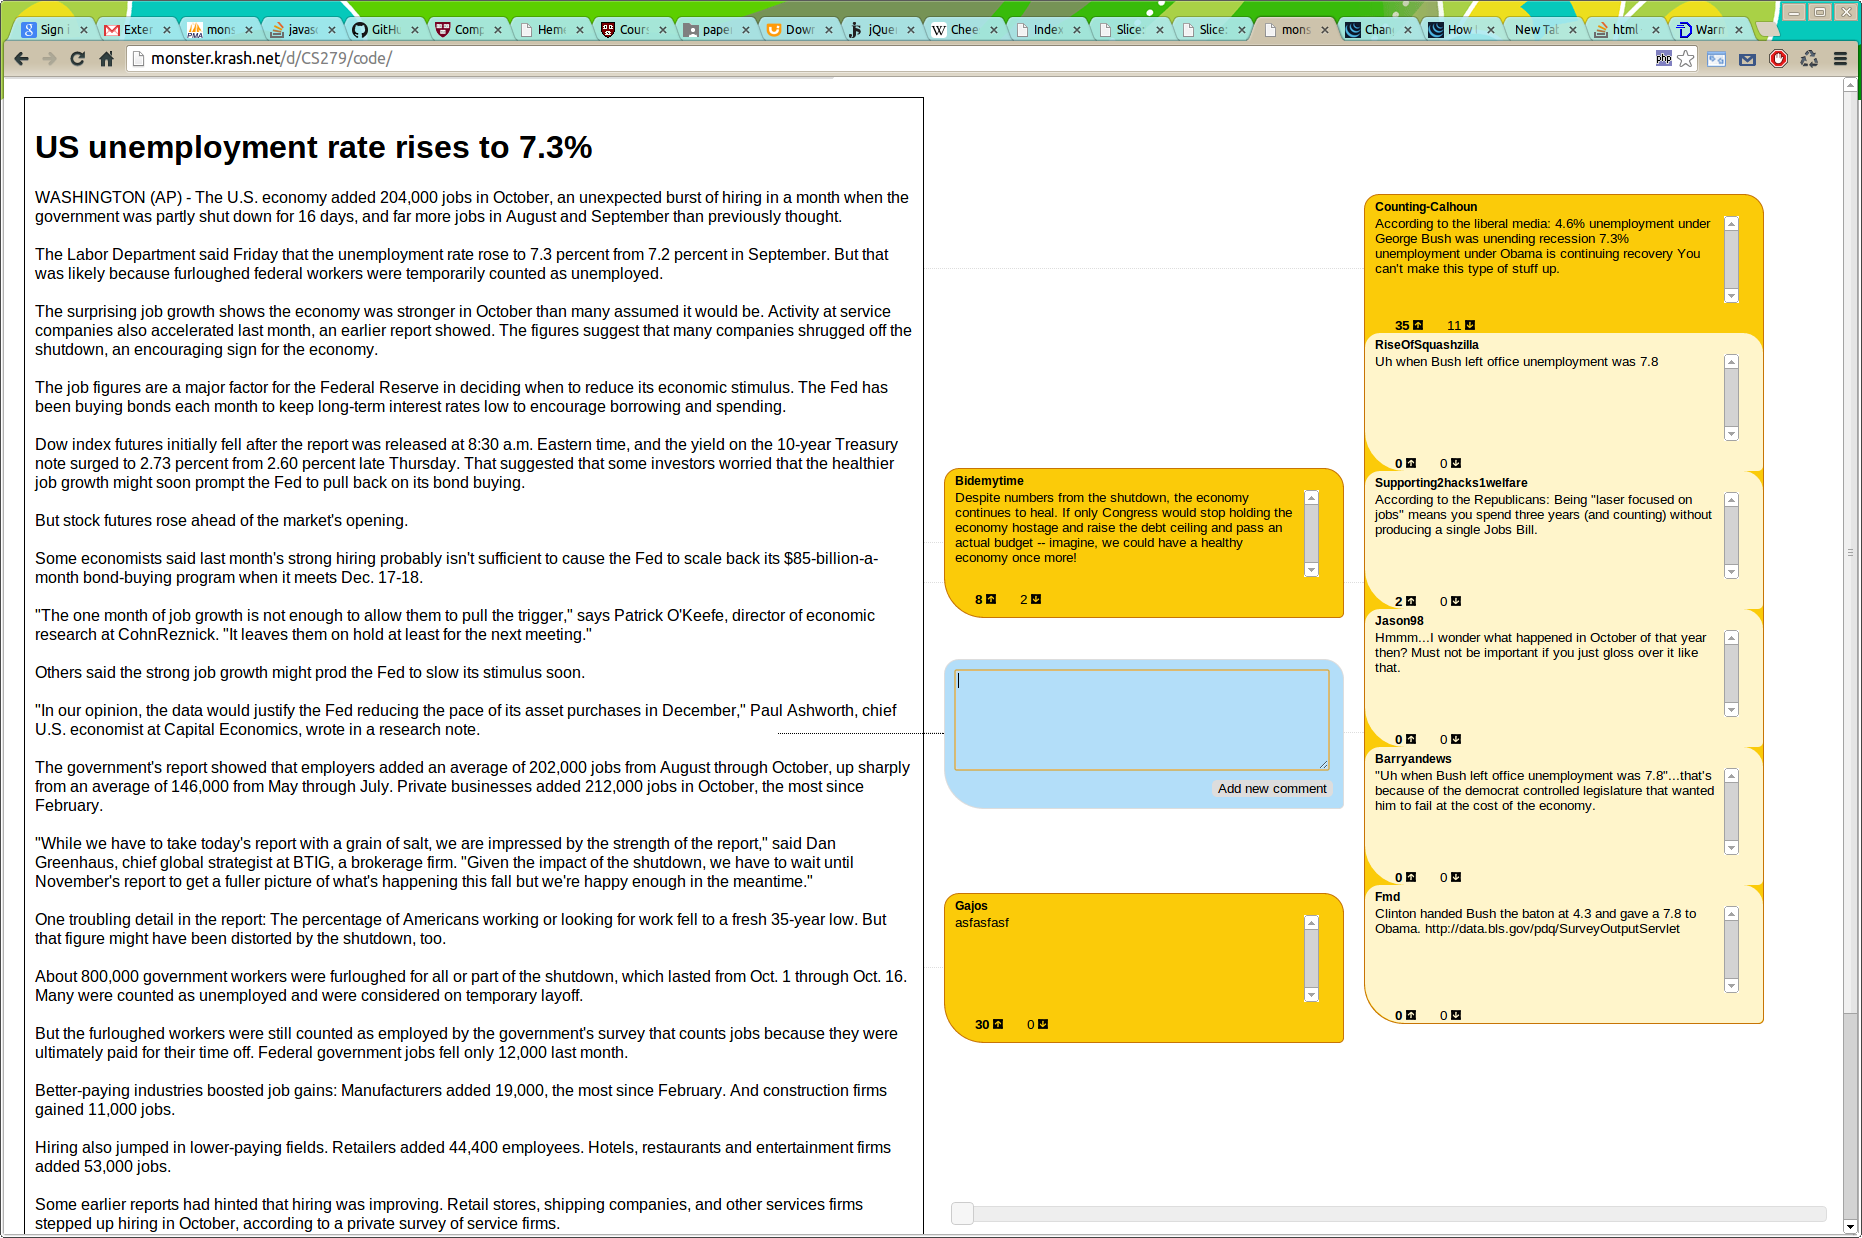
\includegraphics[scale=0.3]{mindmargin.png} 
\caption{The MindMargin system consists of a web client (shown here) and a server side back-end.}
\label{fig:frontend}
\end{figure}

Figure \ref{fig:traditional} shows the traditional vertical commenting system. The reference media is on top and the commenting system is placed below. Navigation within the article as well as within the comments can be performed via top/down scrolling. The organization of replies and up- and down-voting is similar to the MindMargin prototype.

\begin{figure}
\centering
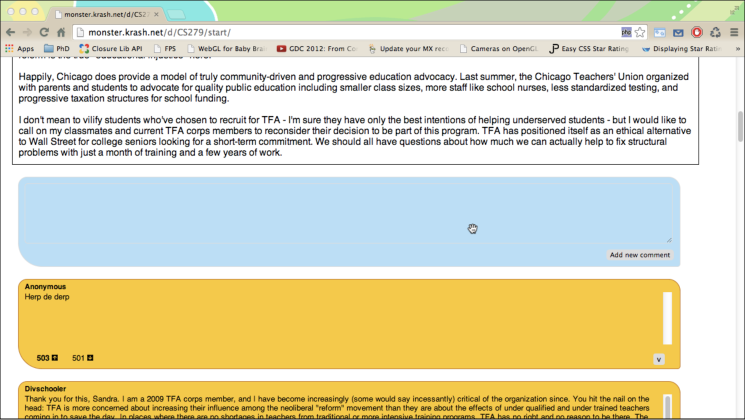
\includegraphics[scale=0.3]{traditional.png} 
\caption{The traditional comment system with a vertically ordered design.}
\label{fig:traditional}
\end{figure}

The front-ends were written in JavaScript using the popular jQuery and jQuery UI libraries. A model-view-controller pattern was chosen to structure the application code base. The user interface itself were created to adjust responsively to any window size.

\subsection{Back-end}
The server component of MindMargin and the traditonal system was written in PHP and communicates with the front-end and a relational database. Communication with the front-end is ensured by providing a REST-API which can be called via AJAX. The entity model of the client is replicated on the server. Data is read and stored using a custom and fully generalized object-relational-mapper. We chose MySQL for our database with a table each for users and comments.

Throughout the implementation, we followed an iterative approach to programming our software. The developer team was small. All developed code is released under the BSD open source license on github.

\section{Experiment}

We performed a blind, online user study with young adults. Participants were randomly assigned to one of two conditions: MindMargin or a vertical commenting interface.

\subsection{Participants}
106 online participants landed on our page for our user study and evaluation, of which 46 proceeded to begin and complete the study (30 female). Participants were recruited online through social media nad college listservs. Participants were college students, aged 18 to 25, and 68 percent hailed from the local university. The self-reported reading frequency of online news among participants ranged from daily to almost never. 

\subsection{Experimental Conditions}
The two conditions in our study were MindMargin and the traditional vertical interface, both seeded with existing comments from a relevant news article. The article was selected on the basis of its opinionated nature and its relevance both in recent news and to our anticipated participant pool. We chose an opinion piece from our university's undergraduate publication, titled “Don’t Teach for America.” 

The article already had over fifty comments by affiliates and non-affiliates of the unversity alike, from which we selected the top 39 comments as ranked by Disqus, the existing commenting system on the publication's website, to be used in our study. The same comments were used in both conditions. In the traditional vertical interface, the comments appeared in the identical order as ranked in the original article. In MindMargin, we anchored them to the article based on textual references, specific phrases, quotes, and relevant content in each comment. 

Users could make new comments by writing in the static new comment box above existing comments in the traditional interface and by clicking any part of the article to open a new comment box in MindMargin. In the MindMargin condition, we provided participants with simple, temporary instructions: "click the text to comment."

XXXX include that last paragraph? XXXX

\subsection{Design and Setup}
We employed a between-subjects test, with participants assigned randomly to one of the two conditions (19 MindMargin). In order to reproduce the conditions under which one would normally read a news article, we chose to recruit participants online and to allow them to self-select themselves into reading the article based on personal time and interest. In order to motivate our participants to actually read or skim the article, instead of skip it, we chose not to use monetary or other time-sensitive incentives. Instead, we chose to design the experiment around the survey question, "Do you (really) think like a student [from our local university]?" 

We then asked participants follow-up questions to verify that they read the article, which included both the overall stance of the article and, in a free-text response, two pieces of supporting evidence used in the article. All 46 participants gave correct and thorough answers to these verification questions. Participants were then asked to complete a post-experiment questionnaire and were not permitted to refer back to the article once the questionnaire was administered.

\subsection{Procedure}
Participants were given an initial questionnaire asking basic demographics and reading frequency. Before given the article, they were also asked either to provide a username or pseudonym, or to remain anonymous. During the reading of the article, participants were allotted 10 minutes. After 2 minutes, they were permitted to proceed to the questionnaire. The 2-minute delay was to ensure the reading of the article, and did not seem to prevent fast readers from moving too slowly, as the average reading time was 3 minutes 47 seconds. 

In the follow-up questionnaire, reading verification questions were first posed. Participants were then asked their personal stance on the article, whether they liked the article, and whether they agreed with the article. They were also asked to self-report whether they read the comments in the article and to provide two adjectives that described either their reaction to, or a description of, the comments.


\section{Results and Discussion}

In this section, we report the findings of our user study that compare the proposed MindMargin interface against the traditional vertical commenting system. Overall, we observed a decrease in polarized views among readers who had seen or read the article previously and an increase in opinion polarization among unfamiliar readers. We also found an increase in readers' positive impressions of comments when using MindMargin. We were able to accept both of our hypotheses.

\subsection{Hypothesis 1}
Our first hypothesis predicted an impact on individual opinions: prompting new readers to develop a stance on an issue and encouraging readers with existing views to consider alternate views. The reasoning behind this hypothesis was that MindMargin exposes readers to a greater number of opinions while reading the article. Consequently, readers think more independently and sharpen their opinions. All participants were asked their stance, from Strongly For TFA to Strongly Against TFA, on a Likert scale. During analysis, we excluded data from participants who reported to have not read the comments (there was no difference in stance between prototypes there). We also excluded participants who did not toggle the Likert scale. The data of the remaining participants (N=XX) was remapped for their "stance extremeness" as $|50 - stance|$ (range 0-50). All participants reported on their familiarity with the article as choices of "none, seen or read". We then performed an analysis for both prototypes including this familiarity with the article as a covarying factor and the dependent variable "stance extremeness SE". We found that there was no significant difference in stance between MindMargin and the traditional commenting system when users did not know the article before. For participants who were familiar, we did observe a difference in individual stance between the prototypes (see figure YYYY). Participants who have seen this article before had a SE of 7 with MindMargin and 17 with the traditional system. Participants who have read this article before had a SE value of 17 with MindMargin and 27 with the traditional system. XXXXXX TODO: talk about p-value here and trend since not significant, also interpretation/discussion XXXXX. Unfortunately, we did not query the participants for their individual stance prior to showing the article which is a limitation of our experiment and will be addressed in future research.



\subsection{Hypothesis 2}
Our second hypothesis predicted an overall increase in positive impressions on comments when using the MindMargin interface. We asked participants who read the comments to input two adjectives in free-text describing either their reaction to the comments or a description of the comments. We then asked four independent volunteers to classify these adjectives using a four-bin classifier ("Positive", "Negative", "Neutral" and "Invalid"). We used the resulting mean encoding to classify the specified adjectives. Then, we compared the impressions between MindMargin and the traditional commenting system. We observed a drastic change of impressions when using MindMargin. As seen in figure \ref{fig:trad_pie}, the majority of participants using the traditional commenting system described the comments as negative (68\%). In contrast, when using MindMargin, the majority of participants described the comments as positive (48\%) or neutral (48\%) as seen in figure \ref{fig:mm_pie}. "Invalid" adjectives were also observed only to occur in the traditional commenting system. XXXX TODO: Ordinal regression? Discussion XXXX We have therefore \textbf{accepted Hypothesis~2}. 

\marginpar{
\begin{figure}
  \begin{center}
  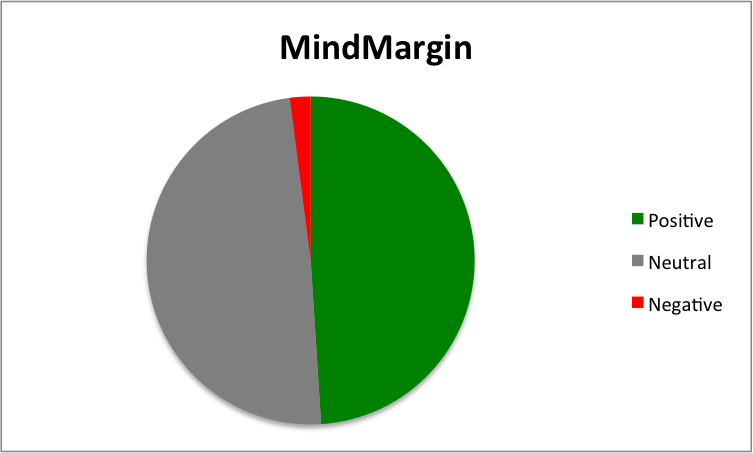
\includegraphics[width=\marginparwidth]{mm_piechart.png}
  \caption{When using MindMargin, the majority of participants described the comments as positive.}
  \label{fig:mm_pie}
  \end{center}
\end{figure}
}

\marginpar{
\begin{figure}
  \begin{center}
  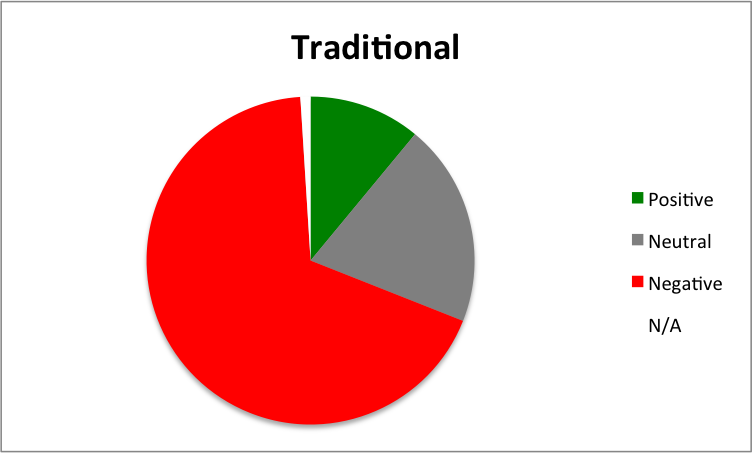
\includegraphics[width=\marginparwidth]{traditional_piechart.png}
  \caption{The majority of participants using the traditional commenting system described the comments as negative.}
  \label{fig:trad_pie}
  \end{center}
\end{figure}
}

In addition to our quantitative results, we would like to quote qualitative feedback from a MindMargin user, suggesting actions he/she took beyond the scope of reading and commenting article: "This article showed me a new perspective on TFA, which after doing research, I have realized I agree with." No feedback suggesting actions outside the scope of the article was received from participants with the traditional commenting system. 

\section{Conclusions}

In this paper, we studied how commenting systems can increase user engagement with comments while reading articles. We report quantitative evidence supporting MindMargin as an interface that depolarizes existing views and establishes new ones by exposing readers to diverse opinions in the comments and that enhances readers' overall impression of existing comments on the article. The key difference between traditional commenting systems and MindMargin is that in the latter, comments are anchored to specific passages of the reference media and are placed on a horizontal infinite scroll. We developed two commenting systems, one using the traditional vertical interface and the other using the MindMargin interface. 

Then, we performed a user study for evaluation. Our key findings include that being exposed to relevant comments during reading increases personal reflection. This results in 10\% less extreme positions regarding the context of the reference article. Additionally, the overall impression of comments significantly diverges. 68\% of users of the traditional commenting system report comments to be negative, while only 2\% of MindMargin users report comments to be negative. 

Future research will include a user study without already seeded comments as well as employ a within-subjects methodology. In addition, we plan to expand the participant pool to include participants of all ages and backgrounds. We would like to explore if MindMargin causes increased difficulty for readers to leave inflamed comments because they must choose an appropriate place to anchor their highly visible comment. Finally, we plan to pursue research on a commenting system like MindMargin, but for videos and music, that anchors comments to certain times or time-intervals within a given recording. Research into annotations on visual pieces, other than text, is also being considered.


\bibliographystyle{acm-sigchi}
\bibliography{lit}
\end{document}
